\chapter{Approach 3: The Financial Genome}

In the previous chapter, we used a set of descriptive words to simultaneously describe features of an account and musical patterns. This technique was used to evaluate the success of the first two implementations.

In this section, we will see how these words can be used to generate a genome which represents an account. We will only go so far as to specify as way of representing this genome, and we will then define a very small genome as a way of demonstrating how this approach will work, and produce a prototype which allows some basic manipulation.

\section{Second Case Study: The Music Genome Project}

In 2006, a group of musicians developed a new way of analysing music. Their aim was to use biological inspiration to classify discrete attributes of music. They called this \textbf{The Music Genome Project}, and used this to produce the successful internet based \textit{Pandora Music} service.\footnote{http://www.pandora.com/mgp.shtml, 21st Feb 2008}

The idea they proposed was to have musicians listen to various pieces of music. They would analyse them by ear, and decide which musical elements (genes) made up the song.

Their ultimate aim was to be able to take the abstract `essences' or `moods' which make up a piece of music, and identify them as something tangible that can be used for classification. This way, when a user likes a specific song, the system can make recommendations to them based on songs with a similar genome.

\section{Notation and Definitions}

\begin{center}
\begin{singlespace}
\begin{tabular}{ l l }
\hline
\textbf{$\vert S\vert$} & The cardinality of S \\ \hline
\textbf{$\mapsto$} & Maplet (maps two elements together) \\ \hline
\textbf{Gene} & An arbitrary unit which determines a characteristic of an account or piece of music \\
\hline
\end{tabular}
\end{singlespace}
\end{center}

\section{Background}

Consider that the approach developed for the \textit{Music Genome Project} can be reversed to generate \textit{music} from \textit{accounts}. If we define a set of genomes, we can then use this as a midway point to map accounts to music. For example, each gene (we will assume a gene has only a single allele) will represent a particular part of some arbitrary music. It will also represent a specific feature in a given account. Added to this, is a set of rules which decide expression rules for sets of genes (transcription rules).

\begin{singlespace}
\begin{formality}
Let $G$ be a single gene \\
Let $A$ be an account consisting of many genes
\end{formality}
\end{singlespace}

\noindent Using the idea of using words to represent the state of an account, we can set up a financial genome for an account as follows:

\begin{singlespace}
\begin{formality}
Let $N_{f}$ be a sequence \\
Let $N_{f}$ be the genome for an account
\end{formality}
\end{singlespace}

\noindent By the same token, we can also have a musical genome given as follows:

\begin{singlespace}
\begin{formality}
Let $N_{m}$ be a sequence \\
Let $N_{m}$ be the genome for music
\end{formality}
\end{singlespace}

\noindent As $N_{f}$ and $N_{m}$ are sequences, the order is important. Take for example the relationship seen in figure \ref{fig:genes}. As elements $N_{f}$ and $N_{m}$ are mapped to specific genes, both sequences need to be specified in the order such that a gene $n$ will be expressed correctly its financial nature in $N_{f}$ and its musical nature in $N_{m}$. The genome from figure \ref{fig:genes} might therefore be sequenced as follows:

\begin{singlespace}
\begin{formality}
$F = \{0 \mapsto null, 1 \mapsto slump, 2 \mapsto soar, 3 \mapsto plunge, 4 \mapsto boom\}$ \\
$N_{a} = \{0 \mapsto null, 1 \mapsto descending, 2 \mapsto ascending\}$ \\
$N_{b} = \{0 \mapsto null, 1 \mapsto major, 2 \mapsto minor\}$ \\
$N_{c} = \{0 \mapsto null, 1 \mapsto scale, 2 \mapsto crescendo, 3 \mapsto chord\}$
\end{formality}
\end{singlespace}

\noindent The intersection of these two sequences' enumeration produces a sequence $N$, which is the general genome. $N_{f}$ and $N_{m}$ are simply expressions (phenotypes) of $\{F, N\}$.

\begin{figure}[ht]
\centering
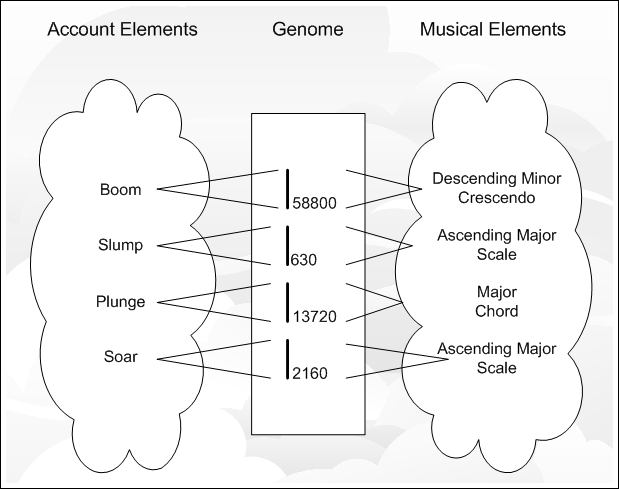
\includegraphics[scale=1.6]{genes}
\caption{Example generated from a simple genome. The genes represent both the features of an account, and also a corresponding musical feature.}
\label{fig:genes}
\end{figure}

\section{Defining Genes}

At the moment, we have a limited system where by an account feature is directly mapped to a musical feature. We can now propose that this system be extended so that an account feature can be mapped to a combination of musical elements.

The first thing that needs to be done is to define rules that take raw numbers, and reduce them to a simple \textbf{account} keyword which describes its overall state.

For example, a decrease in yearly profit from �100,000 to �90,000 is a decrease of 10\%. If we look this up in a `word table', we may find that this corresponds to the word `slump'.

We then define musical sequences in terms of words as well. In this case, I have elected to use two words to describe a musical sequence. For example, the above 10\% decrease in profit corresponds to the word `slump' which is linked to the same genome as the description `descending scale'. This fully defines a gene.

\section{Rules for Defining a Gene}

Below is a table for a specific account (and its generated music), where by each gene has a unique number: \\

\begin{center}
\begin{singlespace}
\begin{tabular}{ | l l l l l | }
\hline
\textbf{Gene \#} & \textbf{Account Wrd} & \textbf{Music Wrd 1} & \textbf{Music Wrd 2} & \textbf{Music Wrd 3} \\ \hline
58800 & Boom & Descending & Minor & Crescendo \\ \hline
630 & Slump & Ascending & Major & Scale \\ \hline
13720 & Plunge & NULL & Major & Chord \\ \hline
2160 & Soar & Ascending & Major & Scale \\
\hline
\end{tabular}
\end{singlespace}
\end{center}

\noindent The gene numbering may seem random upon first glance, but I will show in due course that there is a logical method, and that each combination of words results in a unique gene value. We will now go forward to explain how this genome was generated. We will use the following notation:

\begin{singlespace}
\begin{formality}
Let $A$ be last year�s account \\
Let $B$ be this year�s account \\
Let $F$ be a financial buzz-phrase \\
Let $W1$ be music word 1 \\
Let $W2$ be music word 2 \\
Let $W3$ be music word 3 \\
Let $G$ be a gene \\
Let $GN$ the set of all possible genes for an account
\end{formality}
\end{singlespace}

\noindent We now enumerate $F$ as follows:

\begin{center}
\begin{singlespace}
\begin{tabular}{ | l l | }
\hline
\textbf{Financial Phrase} & \textbf{Enumeration} \\ \hline
NULL & 0 \\ \hline
Slump & 1 \\ \hline
Soar & 2 \\ \hline
Plunge & 3 \\ \hline
Boom & 4 \\
\hline
\end{tabular}
\end{singlespace}
\end{center}

\noindent We also enumerate $W1$ and $W2$ as follows:

\begin{center}
\begin{singlespace}
\begin{tabular}{ | l l l | }
\hline
\textbf{Musical Word} & \textbf{Word ID} & \textbf{Enumeration} \\ \hline
NULL & W1 & 0 \\ \hline
Descending & W1 & 1 \\ \hline
Ascending & W1 & 2 \\ \hline
NULL & W2 & 0 \\ \hline
Major & W2 & 1 \\ \hline
Minor & W2 & 2 \\ \hline
NULL & W3 & 0 \\ \hline
Scale & W3 & 1 \\ \hline
Crescendo & W3 & 2 \\ \hline
Chord & W3 & 3 \\
\hline
\end{tabular}
\end{singlespace}
\end{center}

\noindent We then generate a rule table, a part of which may appear as follows:

\begin{center}
\begin{singlespace}
\begin{tabular}{ | l l | }
\hline
\textbf{ID} & \textbf{Rule} \\ \hline
1 & if $A \textgreater B$ then $W1$ = `Descending' \\ \hline
2 & if $A \leq B$ then $W1$ = `Ascending' \\ \hline
3 & if difference between $A$ and $B$ $\leq$ 10\% then $W2$ = `Scale' \\ \hline
4 & if difference between $A$ and $B$ $\textgreater$ 10\% and $\leq$ 70\% then $W2$ = `Crescendo' \\ \hline
5 & if difference between $A$ and $B$ $\textgreater$ 70\% then $W2$ = `Chord' \\ \hline
\ldots & \ldots \\
\hline
\end{tabular}
\end{singlespace}
\end{center}

\noindent From this table, $W1$ and $W2$ now have values (note, all rules must be processed until both $W1$ and $W2$ have values). We can then assign a unique identity to each gene in our genome. A \textbf{G\"odel Numbering Function} is a suitable way to achieve this, and shows how each combination of words results in a unique identifier:

\begin{singlespace}
\begin{formality}
$G = 2^{F} \cdot 3^{W_{1}} \cdot 5^{W_{2}} \cdot 7^{W_{3}}$
\end{formality}
\end{singlespace}

\noindent The reason for assigning a gene's identity in this way is so that over the processing of many different accounts, common genes can be identified. These genes will always have a unique identifier, and this feature will become incredibly useful if we wish to implement machine learning based on human feedback to decide which genes are expressing themselves the best.

\section{Invalid Genes}

Clearly, some of these genes will be invalid. In the first case, situations such as `ascending chord' simply would not make sense. You will notice that there are several $NULL$ values which can be attributed to a gene. These exist simply so that we can remove any words from a musical description without having to change the structure.\footnote{A Survey of Evolutionary Algorithms for Data Mining and Knowledge Discovery, Alex A. Freitas, section 3.1.2: \url{http://www.macs.hw.ac.uk/~dwcorne/RSR/freitas01survey.pdf}}

Also, due to the nature of the numbering function used, most values will produce genes that cannot be expressed. However, by using a rule table to detect genes, we can be assured that the genome will consist only of valid genes. Any gene enumerations not present in GN cannot be generated from an account by accident.

\section{Gene Expression}

At this point, each set of accounts has a unique genome:

\begin{singlespace}
\begin{formality}
Let $GN$ be the set of all possible genes in the genome (the genome) \\
Let $GN_{n}$ be the genome for account $n$ \\
$GN_{n} \subset GN$
\end{formality}
\end{singlespace}

\noindent Therefore, the genome for the example in \ref{fig:genes} is given as the set $GN_{example} = \{58800, 630, 13720, 2160\}$.

\section{Implementation as a Prototype}

Recall that we have a unique identifier for each gene, generated by enumerating the words and applying the enumeration to a G\"odel numbering function. Because of this, we can make use of Python's \textbf{dictionary} feature. Dictionaries store data in a similar way to lists, but instead of returning an entry via it's \textit{position} in the list, we use a key. This key will be the gene's identifier.

\noindent Here is the syntax for a gene's dictionary entry:

\begin{singlespace}
\begin{formality}
\texttt{\{ geneID: [ 'Financial Keyword', [ 'Direction', 'Key', 'SequenceType' ] ] \}}
\end{formality}
\end{singlespace}

\noindent Therefore, we might have a gene which is defined as:

\begin{singlespace}
\begin{formality}
\texttt{\{ 88200 [ 'Plunge', [ 'Ascending', 'Minor', 'Crescendo' ] ] \}}
\end{formality}
\end{singlespace}

\noindent We also need to specify which word combinations for valid genes. To do this, we define \texttt{W\_VALID} as follows:

\begin{singlespace}
\begin{formality}
\texttt{W\_VALID = [ ( ['Descending', 'Ascending'], ['Major', 'Minor'],}\\
\texttt{['Scale', 'Crescendo'] ), ( ['NULL'], ['Major', 'Minor'], ['Chord'] ) ]}
\end{formality}
\end{singlespace}

\noindent In \texttt{W\_VALID}, each tuple consists of three items. Each of these three items is a list of words. Within each tuple, the valid genes are the set produced by the cartesian product of these lists.

We then call the \texttt{getValidGenes( GN, W\_VALID )} function, which takes in our specification of valid genes, as well as the full genome (\texttt{GN}). It returns a dictionary of just the valid genes.

\section{Gene Encoding}

Encoding the genes requires a simple application of the enumeration we described above. For example, consider the following gene:

\begin{singlespace}
\begin{formality}
\texttt{\{ 1260: [ 'Soar' , [ 'Ascending', 'Major', 'Scale' ] ] }\}
\end{formality}
\end{singlespace}

\noindent Using the encoding we describe, this would result in the following list:

\begin{singlespace}
\begin{formality}
\texttt{[ 2, 2, 1, 1 ]}
\end{formality}
\end{singlespace}

\noindent It then becomes a straight forward matter to perform mutations on single genes, and evolutionary algorithms on gene sets. Seeing as each gene always results in a unique identifier, it is also straight forward to generate a G\"odel number and locate its position in the dictionary. In this way, we can determine whether the mutant is a valid gene or not.

\section{Gene Weightings}

In addition to the current setup, we assign each gene a weight based on its fitness:

\begin{singlespace}
\begin{formality}
Let $W_{n}$ be a sequence containing the weights of genes in account $n$ \\
$\vert W_{n}\vert = \vert GN_{n}\vert$ \\
Let $m$ be the weight multiplier
\end{formality}
\end{singlespace}

\noindent So, as the set $GN$ is built whilst processing the account, a sequence (represented by a list in Python) is built up. The sequence $W_{1}$ corresponding to $GN_{1}$ would be $\langle 1.0, 1.0, 1.0, 1.0 \rangle$ as each of these genes is detected only once.

Let�s say for example, that an account $GN_{2}$ has the same selection of genes as $GN_{1}$, but gene $900$ is detected twice, and gene $54000$ is detected three times. We set $m$ to a constant value of $1.5$. Each weight value is calculated as follows:

\begin{singlespace}
\begin{formality}
Let $G_{n}$ be a gene \\
Let $c$ be the number of times $G_{n}$ is detected \\
The weight of $G_{n}$ is given by $mc-1$
\end{formality}
\end{singlespace}

\noindent In the case of $GN_{2}$, this gives us $W_{2} = \langle1.0, 1.0, 1.5, 2.25\rangle$

\section{Functions of the Prototype}

Below is a full list of functions employed in the prototype:

\begin{singlespace}
\begin{formality}
\texttt{godel( a, b, c, d )}: G\"odel numbering function. \\

\texttt{displayGenome( GN )}: Function to display the genome. \\

\texttt{generateGenes( F\_SET, W1\_SET, W2\_SET, W3\_SET )}: Generate the set of all possible genes. \\

\texttt{getValidGenes( GN, W\_VALID )}: Generate the set of all valid genes (ie, those with valid musical sequences). \\

\texttt{getRandomGeneSet( n, GN\_VALID )}: Produce a random set of genes with n members. \\

\texttt{generateEncoding( gene )}: Generates an encoding for a gene. \\

\texttt{generateEncodings( genes )}: Generates encodings for a set of genes. \\

\texttt{decodeGene( encoding )}: Decodes a gene. \\

\texttt{decodeGenes( encodings )}: Decodes several genes. \\

\texttt{mutateGene( gene, validGenes )}: Performs an single-random-gene new-allele mutation given an encoding. \\

\texttt{mutateGeneSet( genes, m, validGenes )}: Performs an m-random-gene new-allele mutation on a set of genes. \\

\texttt{generateGenomeWeights( genome )}: Generate evenly distributed weights for a genome. \\

\texttt{increaseWeight( encodedGene, weights )}: Increase the weight of a gene.
\end{formality}
\end{singlespace}

\noindent The prototype operates by calling functions from within the Jython interpreter in order to perform the operations.

\section{Beyond the Prototype}

Due to time constraints, the prototype was not developed beyond its current state. The next stage would have involved plugging the genome into one of the first two implementations. A population would have been generated for an account, and its fitness evaluated in relation to the music produced. A number of experts would have been required to make this a reality.

\section{Summary}

In this, the penultimate chapter, we have seen how we can use words to describe both accounts and music. By using the cartesian product, we can produce a genome set which covers all mapping possibilities of accounts to music. The evaluation of the fitness of these genes is the domain of financial experts and musicians, and these resources lie outside the scope of this project.

Over the previous chapters, we have looked at two full implementations and one prototype. In the next chapter, we will sum up and see what conclusions have been reached from this project.






